\subsubsection*{Doxygen's internals}

{\bf Note that this section is still under construction!}

The following picture shows how source files are processed by doxygen.

\begin{Image}
\begin{center}
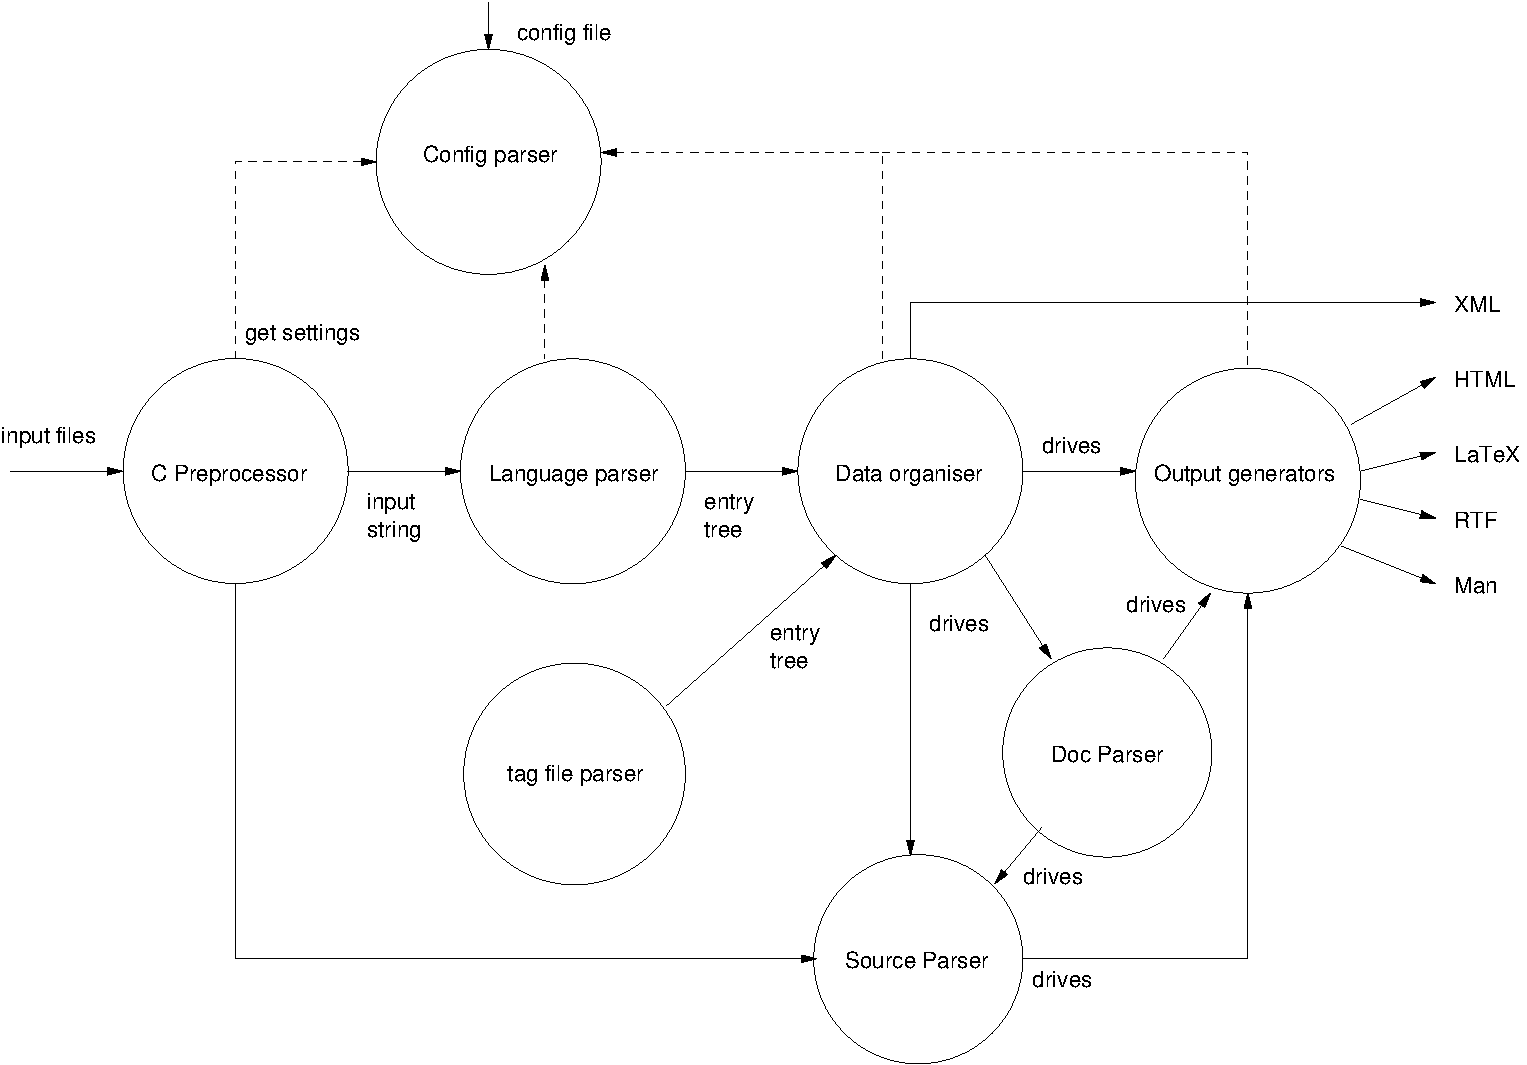
\includegraphics[width=14cm]{archoverview}\caption{Data flow overview}
\end{center}
\end{Image}


The following sections explain the steps above in more detail.

\subsubsection*{Config parser}

The configuration file that controls the settings of a project is parsed and the settings are stored in the singleton class {\tt Config} in {\tt src/config.h}. The parser itself is written using {\tt flex} and can be found in {\tt src/config.l}. This parser is also used directly by {\tt doxywizard}, so it is put in a separate library.

Each configuration option has one of 5 possible types: {\tt String}, {\tt List}, {\tt Enum}, {\tt Int}, or {\tt Bool}. The values of these options are available through the global functions {\tt Config\_\-getXXX()}, where {\tt XXX} is the type of the option. The argument of these function is a string naming the option as it appears in the configuration file. For instance: {\tt Config\_\-getBool}(\char`\"{}GENERATE\_\-TESTLIST\char`\"{}) returns a reference to a boolean value that is {\tt TRUE} if the test list was enabled in the config file.

The function {\tt readConfiguration()} in {\tt src/doxygen.cpp} reads the command line options and then calls the configuration parser.

\subsubsection*{C Preprocessor}

The input files mentioned in the config file are (by default) fed to the C Preprocessor (after being piped through a user defined filter if available).

The way the preprocessor works differs somewhat from a standard C Preprocessor. By default it does not do macro expansion, although it can be configured to expand all macros. Typical usage is to only expand a user specified set of macros. This is to allow macro names to appear in the type of function parameters for instance.

Another difference is that the preprocessor parses, but not actually includes code when it encounters a \#include (with the exception of \#include found inside \{ ... \} blocks). The reasons behind this deviation from the standard is to prevent feeding multiple definitions of the same functions/classes to doxygen's parser. If all source files would include a common header file for instance, the class and type definitions (and their documentation) would be present in each translation unit.

The preprocessor is written using {\tt flex} and can be found in {\tt src/pre.l}. For condition blocks (\#if) evaluation of constant expressions is needed. For this a {\tt yacc} based parser is used, which can be found in {\tt src/constexp.y} and {\tt src/constexp.l}.

The preprocessor is invoked for each file using the {\tt preprocessFile()} function declared in {\tt src/pre.h}, and will append the preprocessed result to a character buffer. The format of the character buffer is



\footnotesize\begin{verbatim}
0x06 file name 1 
0x06 preprocessed contents of file 1
...
0x06 file name n
0x06 preprocessed contents of file n
\end{verbatim}
\normalsize


\subsubsection*{Language parser}

The preprocessed input buffer is fed to the language parser, which is implemented as a big state machine using {\tt flex}. It can be found in the file {\tt src/scanner.l}. There is one parser for all languages (C/C++/Java/IDL). The state variables {\tt insideIDL} and {\tt insideJava} are uses at some places for language specific choices.

The task of the parser is to convert the input buffer into a tree of entries (basically an abstract syntax tree). An entry is defined in {\tt src/entry.h} and is a blob of loosely structured information. The most important field is {\tt section} which specifies the kind of information contained in the entry.

Possible improvements for future versions:\begin{itemize}
\item Use one scanner/parser per language instead of one big scanner.\item Move the first pass parsing of documentation blocks to a separate module.\item Parse defines (these are currently gathered by the preprocessor, and ignored by the language parser).\end{itemize}


\subsubsection*{Data organizer}

This step consists of many smaller steps, that build dictionaries of the extracted classes, files, namespaces, variables, functions, packages, pages, and groups. Besides building dictionaries, during this step relations (such as inheritance relations), between the extracted entities are computed.

Each step has a function defined in {\tt src/doxygen.cpp}, which operates on the tree of entries, built during language parsing. Look at the \char`\"{}Gathering information\char`\"{} part of {\tt parseInput()} for details.

The result of this step is a number of dictionaries, which can be found in the Doxygen \char`\"{}namespace\char`\"{} defined in {\tt src/doxygen.h}. Most elements of these dictionaries are derived from the class {\tt Definition}; The class {\tt MemberDef}, for instance, holds all information for a member. An instance of such a class can be part of a file ( class {\tt FileDef} ), a class ( class {\tt ClassDef} ), a namespace ( class {\tt NamespaceDef} ), a group ( class {\tt GroupDef} ), or a Java package ( class {\tt PackageDef} ).

\subsubsection*{Tag file parser}

If tag files are specified in the configuration file, these are parsed by a SAX based XML parser, which can be found in {\tt src/tagreader.cpp}. The result of parsing a tag file is the insertion of {\tt Entry} objects in the entry tree. The field {\tt Entry::tagInfo} is used to mark the entry as external, and holds information about the tag file.

\subsubsection*{Documentation parser}

Special comment blocks are stored as strings in the entities that they document. There is a string for the brief description and a string for the detailed description. The documentation parser reads these strings and executes the commands it finds in it (this is the second pass in parsing the documentation). It writes the result directly to the output generators.

The parser is written in C++ and can be found in src/docparser.cpp. The tokens that are eaten by the parser come from src/doctokenizer.l. Code fragments found in the comment blocks are passed on to the source parser.

The main entry point for the documentation parser is {\tt validatingParseDoc()} declared in {\tt src/docparser.h}. For simple texts with special commands {\tt validatingParseText()} is used.

\subsubsection*{Source parser}

If source browsing is enabled or if code fragments are encountered in the documentation, the source parser is invoked.

The code parser tries to cross-reference to source code it parses with documented entities. It also does syntax highlighting of the sources. The output is directly written to the output generators.

The main entry point for the code parser is {\tt parseCode()} declared in {\tt src/code.h}.

\subsubsection*{Output generators}

After data is gathered and cross-referenced, doxygen generates output in various formats. For this it uses the methods provided by the abstract class {\tt OutputGenerator}. In order to generate output for multiple formats at once, the methods of {\tt OutputList} are called instead. This class maintains a list of concrete output generators, where each method called is delegated to all generators in the list.

To allow small deviations in what is written to the output for each concrete output generator, it is possible to temporarily disable certain generators. The OutputList class contains various {\tt disable()} and {\tt enable()} methods for this. The methods {\tt OutputList::pushGeneratorState()} and {\tt OutputList::popGeneratorState()} are used to temporarily save the set of enabled/disabled output generators on a stack.

The XML is generated directly from the gathered data structures. In the future XML will be used as an intermediate language (IL). The output generators will then use this IL as a starting point to generate the specific output formats. The advantage of having an IL is that various independently developed tools written in various languages, could extract information from the XML output. Possible tools could be:\begin{itemize}
\item an interactive source browser\item a class diagram generator\item computing code metrics.\end{itemize}


\subsubsection*{Debugging}

Since doxygen uses a lot of {\tt flex} code it is important to understand how {\tt flex} works (for this one should read the man page) and to understand what it is doing when {\tt flex} is parsing some input. Fortunately, when flex is used with the -d option it outputs what rules matched. This makes it quite easy to follow what is going on for a particular input fragment.

To make it easier to toggle debug information for a given flex file I wrote the following perl script, which automatically adds or removes -d from the correct line in the Makefile:



\footnotesize\begin{verbatim}
#!/usr/local/bin/perl 

$file = shift @ARGV;
print "Toggle debugging mode for $file\n";

# add or remove the -d flex flag in the makefile
unless (rename "Makefile.libdoxygen","Makefile.libdoxygen.old") {
  print STDERR "Error: cannot rename Makefile.libdoxygen!\n";
  exit 1;
}
if (open(F,"<Makefile.libdoxygen.old")) {
  unless (open(G,">Makefile.libdoxygen")) {
    print STDERR "Error: opening file Makefile.libdoxygen for writing\n";
    exit 1; 
  }
  print "Processing Makefile.libdoxygen...\n";
  while (<F>) {
    if ( s/\(LEX\) -P([a-zA-Z]+)YY -t $file/(LEX) -d -P\1YY -t $file/g ) {
      print "Enabling debug info for $file\n";
    }
    elsif ( s/\(LEX\) -d -P([a-zA-Z]+)YY -t $file/(LEX) -P\1YY -t $file/g ) {
      print "Disabling debug info for $file\n";
    }
    print G "$_";
  }
  close F;
  unlink "Makefile.libdoxygen.old";
}
else {
  print STDERR "Warning file Makefile.libdoxygen.old does not exist!\n"; 
}

# touch the file
$now = time;
utime $now, $now, $file
\end{verbatim}
\normalsize
 